\documentclass[a4paper,11pt]{report}
\usepackage[latin1]{inputenc}
\usepackage[english]{babel}
\usepackage{graphicx}
\usepackage{pdfpages}
\usepackage{fancyvrb}
\usepackage{fancybox}
\usepackage{listings}
\usepackage{color}
\usepackage{framed,color}
\usepackage{textcomp}
\usepackage{url}
\bibliographystyle{ieeetr}
\begin{document}

% listing styles
\lstset{numbers=left, numberstyle=\tiny,basicstyle=\ttfamily\scriptsize, tabsize=2,
keywordstyle=\underbar, stringstyle=\small, backgroundcolor=\color[gray]{0.94},
framexleftmargin=2pt}
\lstdefinestyle{rdfa}{numberblanklines=true, morekeywords={}}

% Turtle box
\definecolor{olivegreen}{rgb}{0.2,0.8,0.5}
\definecolor{grey}{rgb}{0.5,0.5,0.5}
\lstdefinelanguage{ttl}{
sensitive=true,
morecomment=[l][\color{grey}]{@},
morecomment=[l][\color{olivegreen}]{\#},
morestring=[b][\color{blue}]\",
keywordstyle=\color{cyan},
morekeywords={version,owl,rdf,rdfs,xml,xsd,dbpedia,dbo,str,sso,scms,fr,ld}
}

\lstset{
        basicstyle=\ttfamily\scriptsize,
        upquote=true,
        showspaces=false,
        showstringspaces=false,
        showtabs=false,
        tabsize=2,
        frame=none,
        breaklines,
        numbers=none,
        framexleftmargin=2mm,
        xleftmargin=2mm,
}

\begin{titlepage}
\begin{center}

\includegraphics[width=5cm]{EURECOM_logo_quadri}
\\[3cm]
\textbf{\Huge{EventSpotter}}
\\[0.2cm]
\textbf{\textsc{\LARGE{spotting entities that talk about events}}}
\\[2cm]
\textbf{\textsc{\LARGE{Project Report}}}
\\[0.5cm]
\LARGE{Amar Kadamalakunte , Meghana Sreekanta Murthy}
\\[0.1cm]
\large{Fall 2012 - Spring 2013}
\\[7.92cm]
\columnsep3cm
\begin{tabular}{p{8cm} p{8.5cm}}
\small{\textbf{Supervisors:}\newline
Rapha\"el Troncy\newline
Giuseppe Rizzo}
&
\small{\textbf{EURECOM\newline Multimedia Department}}
\end{tabular}
\end{center}
\end{titlepage}


 \tableofcontents

\chapter*{Abstract}
By definition, an event is an occurrence in the past, present or future. Events could be classified as musical events, sports events, news events, etc. The aim of our work is to develop an approach to spot the existence of musical event entities in free form text. The EventSpotter uses a large dataset called EventMedia to identify candidate event spots in the text, and disambiguates them by assigning a confidence score. The confidence score itself is based on the identification of correlated entities (event location or artists) in the surrounding text and cosine similarity measure between the surrounding text and existing description of event in the dataset. We used Precision, Recall and F-measure to evaluate our approach using the ubiquitous CoNLL eval method for evaluation. We used event description from the EventMedia dataset as input and found that the EventSpotter performed better than some exisiting approaches for event detection in the musical domain. We present our method and findings in this paper.
\addcontentsline{toc}{chapter}{Abstract}

\chapter*{1 Introduction}
\addcontentsline{toc}{chapter}{1 Introduction}
\section*{1.1 Motivation}
In today's day and age, we are surrounded by a plethora of events, some of them are planned, organized and conducted whereas some of them are unplanned occurrences such as natural calamities. These events can be formally classified as ``Planned'' or ``Scheduled'' events and ``Unplanned'' or ``Breaking-news'' events. The EventSpotter project is aimed at detecting ``planned'' event entities in text. Social event sharing websites such as last.fm, Eventful and Upcoming contain the most precise and up to date information related to scheduled or planned events. In this paper we present a novel approach that attempts to use this social data to spot event entities by combining various NLP and machine learning techniques. EventSpotter has been developed as an application which uses live social event data stream aggregated from various sources in the Web. This task, of scraping the Web for event data, is performed by EventMedia\cite{EURECOM+3865}. A snapshot of the EventMedia dataset is taken and used as an event lexicon for the EventSpotter. Every time there is a change affected to the EventMedia dataset an update of the event lexicon is triggered. Thus by relying on a live social data stream we demonstrate that our approach can overcome the static nature of other rigid rule based approaches such as Conditional Random Field classifiers. In our approach we first use the social event data to identify candidate events, then disambiguate these candidate spots using event attributes such as artists, venue, date, event description and category. and assign a confidence score based on a cosine similarity with the event descriptions from EventMedia. 
\addcontentsline{toc}{section}{1.1 Motivation}

\section*{1.2 Challenges for Entity Extraction in the Event Domain}

The complexity of entity extraction increases manifold in the event domain. The biggest challenge of this task is to obtain a clear unambiguous definition of an event title. This is because there is a lack of uniform rule based nomenclature with respect to events. For instance, it is common practice for musical events to be named after the artists who are performing at the event (see example 1.1). Here, the event title is ``Beth Jeans Houghton '' which is also the name of the performing artist. This brings in a word sense disambiguation problem, where the onus is on comprehending whether the spot refers to the artist or to the event. The next level of complexity is introduced when an event title is created as an amalgamation of the artist names, band names, event venue and at times even the date, using special characters (see example 1.2). Here, ``Stay Sharp Album Release Party: Higher Hands + Grilled Lincolns + Pressing Strings'' is an event title as per the information uploaded on the event sharing website ``eventful''. In essence this means any stripping or stop-wording of input text, which would have otherwise been a natural choice for a preprocessing step in any information extraction problem, is completely out of question. This also means the length of an event title may range from just one word to a phrase with many words and punctuations. Further, at times the boundaries of creative license are stretched to the point where events are named with words that don''t even exist in the language vocabulary (see example 1.3). Here, ``Pocktoberfest'' is an yearly event which takes place at the ``Pocklington arts center''. But the word ``Pocktoberfest'' does not exist in the English language. If all events followed a standard naming scheme, our task which now seems herculean, would have been average, at best.\newline 

\begin{lstlisting}[caption=This listing shows different ways in which event titles are constructed., label=amb]
Example 1.1

In the input``Beth Jeans Houghton & THE HOOVES OF DESTINY, Yours Truly Cellophane Nose introduces one of the most self-assured new artists of the year a pop polymath whose blend of psychedelia glam rock and chain gang folk is quite unlike anything else you are likely to hear in 2012.'', the event title is ``Beth Jeans Houghton''.

Example 1.2

``Stay Sharp Album Release Party: Higher Hands + Grilled Lincolns + Pressing Strings''is an event title characterised by 3 band names.

Example 1.3

``Pocktoberfest'' is an event title that is comprises of words that are not present in the language vocabulary.
\end{lstlisting}

While in some cases it makes sense to rely on the semantic meaning to detect the presence of an event entity, in other cases a posteriori knowledge of event titles could prove to be more useful.  Due to this heterogeneity in nomenclature, it gets exceedingly difficult even for humans to identify event entities in text, let alone information extraction softwares.  Clearly, this shows that the problem of event entity extraction is too complex to be solved by just a linguistic approach or a static knowledge based approach. In this paper we explore the plausibility of using a mixture of various NLP and machine learning techniques to event detection and demonstrate that it is possible to obtain an increase in recall even with a linear combination of linguistic and knowledge based approaches. The highlight of the EventSpotter project is the proposition of a novel approach which leverages a live stream of social event data to detect event entities in text. In the following sections, we first discuss the emergence of popular trends in the domain of entity extraction and how they influenced our work, then we take a detailed look at the EventSpotter approach, the golden dataset creation, usage of 10-fold cross validation to evaluate the performance of the system and conclude with our thoughts on how we can potentially better the performance of the EventSpotter with the help of machine learning techniques.
\addcontentsline{toc}{section}{1.2 Challenges for Entity Extraction in the Event Domain}
%\section*{Contents}

\chapter*{2 Related Work}
\addcontentsline{toc}{chapter}{2 Related Work}

\section*{2.1 Trends in the Event Entity Extraction Domain}
Many people have tried to tackle the problem of entity detection in the past. While some have relied purely on the linguistic properties of text others have used context and domain knowledge to accurately detect entities. In \cite{Gruhl_contextand} we came across one such approach that inspired us during the literature survey phase of the EventSpotter. In this case, the utilisation of context and domain knowledge along with the application of real world constraints proved to be beneficial in improving the accuracy of entity detection. The main goal was to establish semantic relationships between entities in social networking and content sharing sites like MySpace and Youtube. In this approach, the authors used an edit-distance based spotter to match the knowledge base with the text taken from online forums discussing popular music. They then checked for domain and context information and applied an SVM classifier. Further, a study of \cite{Hassell06ontology-drivenautomatic} introduced us to the approach of identifying entities based on knowledge from populated ontologies such as DBWorld and DBLP. They used clues such as entity names, text-proximity, text co-ocurrence, popularity of entities, semantic relationships between entities for disambiguation. This approach further vindicated our idea of using the large EventMedia knowledge base to detect events in EventSpotter.\newline

As part of another approach, DBpedia URIs were used for automatic annotation of texts. The DBpedia Spotlight \cite{Mendes11dbpediaspotlight:} used an extensive ontology with 272 classes, called DBpedia, and also provided the flexibility of choosing domain of interest. 2 sources of textual references include: the lexicon created from the DBpedia graph (of labels, redirects, disambiguations) and wikilinks. The EventSpotter derives various facets of the DBpedia Spotlight approach including the 4 main stages: (1)Spot phrases that may indicate a mention of a DBpedia resource, (2)Select candidates by spotted phrase-to-resources mapping, (3)Disambiguate by using the context around spotted phrase, (4)Configure the annotation by customization from user with Resource Prominence, Topic Pertinence, Contextual Ambiguitvalidy, Disambiguation Confidence. We also studied two interesting methodologies that were applied to social media and wikipedia for detection of events. TWICAL \cite{Ritter_opendomain} focused on linguistic properties and temporal expressions to detect events, classified them using the context of surrounding phrases and finally ranked them according to strong associations with a unique date. The Wikipedia Live Monitor\cite{DBLP:journals/corr/abs-1303-4702} tracked edits on various linguistic versions of a single document on wikipedia and relied on cross-language, full-text search across social networks in order to evaluate the \cite{Hassell06ontology-drivenautomatic} plausability of the edits being events. \newline

Although the above mentioned approaches are effective in entity spotting, there are a few limitations within each. In \cite{Gruhl_contextand}, the authors cite the absence of a training corpus and regions of text being commonly used words, as limiting factors. They also speak of the ambiguous nature of song titles being a major limitation. In \cite{Hassell06ontology-drivenautomatic} the non-exhaustive nature of any knowledge base proves to be the biggest hurdle. The same is the case with the DBpedia spotlight approach defined in \cite{Mendes11dbpediaspotlight:}, where the authors do not speak of using linguistic tools such as a Conditional Random Field classifier to detect entities that are non existent in the knowledge base. Both TWICAL \cite{Ritter_opendomain} and Wikipedia Live monitor \cite{DBLP:journals/corr/abs-1303-4702} are dependant on social networking sites to detect events. As a result, events that are not publicised in the social networking domain go undetected. The fact that each of these approaches have limitations of their own, goes to show that there is still scope for improvement in the field of event detection. The EventSpotter project is an attempt to meet this need for a more complete approach towards event detection.

\addcontentsline{toc}{section}{2.1 Trends in the Event Entity Extraction Domain}
\section*{2.2 BookSpotter}

BookSpotter Enhancement Engine by Sztaki\footnote{http://blog.iks-project.eu/introducing-bookspotter-enhancement-engine-by-sztaki/} takes a knowledge based approch to find book occurrences within text. It loads a list of titles into memory and matches them with tokens of input text to spot book occurrences. It further disambiguates each spot using the author string stored in a database. If one or more authors are present in the text, the spot is considered a valid one. The BookSpotter enhancement engine is designed to work as a module inside Apache Stanbol\footnote{http://stanbol.apache.org/}. Apache Stanbol provides a set of reusable components for semantic content management. The BookSpotter uses Stanbol for presenting the detected entities as RDF. We were greatly inspired by the idea behind the BookSpotter project. We spent a considerable amount of time analysing and understanding the logic of the BookSpotter system. In a way, the EventSpotter project stands upon the shoulders of BookSpotter. We supplement the logic of the BookSpotter with event-specific feature verifications, such as presence of: artists, venue, date, event description and category.

\addcontentsline{toc}{section}{2.2 BookSpotter}


\chapter*{3 Approach}
The EventSpotter approach has four stages namely: (1)Preprocessing, (2)Candidate selection, (3)Disambiguation and (4)Postprocessing. It is imperative to restate that we have reused components of the BookSpotter which act as a foundation on which the EventSpotter is built on.

\addcontentsline{toc}{chapter}{3 Approach}
\section*{3.1 Overview}
Before we look at each of these in greater detail, it is important to first gain a high level understanding of the entire system.
\begin{figure}
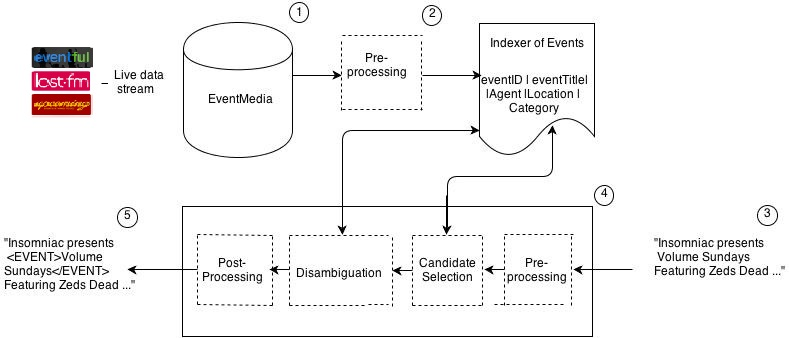
\includegraphics [width=13cm,height=6cm]{architecture}
\caption{EventSpotter system}
\end{figure}

\addcontentsline{toc}{section}{3.1 Overview}

\subsection*{3.1.1 EventMedia Dataset}
EventMedia is a huge hub of social event data obtained from three public event directories: Last.fm, Eventful and Upcoming and the media directory: Flickr. In \cite{EURECOM+3865}, EventMedia is described to be a platform that uses semantic Web technologies to aggregate and interlink real-time heterogeneous data sources. Information within EventMedia is in the form of encapsulated media and eventdescriptions, which are supported by background knowledge from data sources such as DBpedia, MusicBrainz, BBC and Foursquare. 

We retrieved a snapshot of the EventMedia database which constituted 67957 events. This snapshot, taken on the 26th of November 2012, contains metadata for events that occurred during the year 2012. Each event in the EventMedia snapshot has the following attributes: eventId(url to a web page corresponding to the event in data.linkedevents.org), eventTitle, publisher, date, locations, category, agent(artists or bands performing at the event) and event description. We provide in the listing given below, an example of a sample record from the EventMedia dataset. The events belonged to one or more of the following categories: Musical Concert, Festivals, Nightlife, Social Gathering, Performing Arts, Visual and Performing Arts, Movies, Visual Arts, Food, Neighborhood, Community, Religion and Spirituality, Museums and Attractions, Outdoors Recreation, Family and Kids, Galleries and Exhibits, Professional, Fundraising and Charity, Commercial and Sales, Education, Sports, Organizations and Meetups, Business and Networking, Politics, Media and Literary, Health and Wellness, Life Style, Conferences and Tradeshows, On Campus, Science, Technology, Animals, Comedy, Other and Miscellaneous. \newline 

\begin{lstlisting}[caption = This listing shows an example of a sample record from the EventMedia dataset.]
eventId : http://data.linkedevents.org/event/143561b1-08ab-4970-9873-f80d232ccc07
eventTitle : Lights
publisher : http://www.last.fm
date : 2012-02-24 19:00:00
location : Scala
category : Musical Concert
agent : Nightbox
eventDescription : The event was moved to Scala!
\end{lstlisting}

For the EventSpotter implementation, we used a modified version of the EventMedia Dataset, as shown in step 1 of the figure. We found, upon investigation, that it was necessary to merge multiple records pertaining to the same eventID. The reason why we chose to address this issue was because, when we used the EventMedia dataset as is, redundant event identifications were created. It is imperitive to note that though these recoreds share the same ID, they differ from time to time in category or agent attributes. In order to tackle this problem, we created event objects for each record, compared their event IDs and merged those objects that had matching eventIDs. Thus during the merge operation, multiple records were transformed into a single record that contained a list of agent strings and list of category strings rather than a single agent string and a single category string. Finally we created a comma separated value (.csv) file that was exported into MySQL. By performing such an operation, the number of records in the new dataset reduced to 34195.   
 
\addcontentsline{toc}{subsection}{3.1.1 EventMedia Dataset}

\subsection*{3.1.2 EventTitles}
EventTitles.list file can be considered an event indexer or lexicon which contains, as the name suggests, titles of all events listed in the EventMedia database, mapped to their corresponding eventId. This file is loaded onto memory at the beginning of the execution.
\addcontentsline{toc}{subsection}{3.1.2 EventTitles}

As seen in the figure, the EventSpotter spots candidate entities by matching input text with the indexer of events which is also known as the eventtitles file, and then validates these spots using the agent and location fields from the EventMedia dataset.

\section*{3.2 Preprocessing}

The preprocessing stage mainly comprises of 2 phases, where we first follow a method of text tokenization common to both phases and then a method of sentensization which is unique only to the 2nd phase. The first phase of preprocessing, as indicated by step 2 in the figure, is performed on the information extracted from EventMedia. Here, we perform solely tokenization to divide the attributes such as event title, agent etc. into distinct components. The second phase of preprocessing is an integral part of the 4 stage approach of the EventSpotter and is performed on the input text obtained from the user. As indicated in step 3 of the figure the input text could look like ``Insomniac presents Volume Sundays Featuring Zeds Dead...''.  As mentioned previously, our tokenizer's main role here is to similarly divide the entire text provided to it by the user into a set of distinct tokens. This tokenizing process during both phases ensures that there is no scope for any mismatch because of inconsistencies in the matchable string information from EventMedia and the input. Additionally, in the 2nd phase of the preprocessing step, we also carry out a process called ``sentensize'' where the entire input text is divided into a a set of sentences, instead of just tokens. The objective of this process is to ensure the availability of distinct sentences for the later stage of Disambiguation, where we use the sentences to create surrounding information for a candidate event spot. Example 3.1 shows that the text is broken into sentences by considering various line terminations such as ``.'' dot, ``!'' exclaimation, ``?'' question mark etc.
EventSpotter uses the java.util.Locale library for this operation. This stage and the following 3 stages of core EventSpotter logic are indicated together as step 4 in the figure. \newline
\newline
\newline
\newline
\begin{lstlisting}[caption=This listing shows how sentensization works in EventSpotter]
Example 3.1

Input:
``Tickets on sale now. Doors open: 6:30PM Showtime: 7:30PM  Minus the Bear  comes to The Depot November 6th with special guests Cursive & Girl in a Coma! Tickets available at all Smith's Tix locations, have you booked your seats yet?''

Output:
sentences
{
``Tickets on sale now.'', 
``Doors open: 6:30PM Showtime: 7:30PM  Minus the Bear  comes to The Depot November 6th with special guests Cursive & Girl in a Coma!'',
``Tickets available at all Smith's Tix locations, have you booked your seats yet?''
}
\end{lstlisting}

\addcontentsline{toc}{section}{3.2 Preprocessing}

\section*{3.3 Candidate Selection}

For every input text token that was derived from the tokenization phase of the preprocessing stage, EventSpotter checks for a case-insensitive match with the tokenized version of the indexer of events or eventtitles file. The reason for performing such a case insensitive match is to ensure that we encompass all candidate event names, without losing any because of an insignificant case-sensitive mismatch. We call this type of mismatch insignificant because of the fact that since we consider unstructured input text, it is quite possible that event names may not be highlighted consistently in the same manner of case. For instance, the input text could be represented in different ways for a single event title. For instance an event title can be mentioned as ``Volume Sundays''(see example 4.1), ``VoLume SUNDAYS''(see example 4.2) and ``VOLUME SUNDAYS''(see example 4.3) in an input text. Since all 3 cases refer to the event ``Volume Sundays'', they  should be ideally selected. With this in mind we refrained from performing an exact string match. Our aim was to start with the largest set of candidate events and gradually limit the set to confirmed events by disambiguation. When a match occurs, the string of tokens are concatenated to a list named Matches. As understood, this list contains all string matches that have occured during one complete cycle of the EventSpotter. EventSpotter checks further in Matches and considers only those strings that either start with a capital letter or a digit, as candidate events. By analysis of the event names in  EventMedia, we understood that the most probable events were usually pronouns starting with a capital letter or a digit. \newline 

\begin{lstlisting}[caption= This listing shows different representations of input text for a single event title.]
Example 4.1
``Insomniac presents Volume Sundays Featuring Zeds Dead...''

Example 4.2
``Insomniac presents VoLume SUNDAYS Featuring Zeds Dead...'' 

Example 4.3
``Insomniac presents VOLUME SUNDAYS Featuring Zeds Dead...''.
\end{lstlisting}

\addcontentsline{toc}{section}{3.3 Candidate Selection}

\section*{3.4 Disambiguation}

In this stage we ascertain the validity of each entry in the candidate list with the help of metadata stored in the EventMedia dataset. Here we make an important hypothesis: it is prudent, for a knowledge based approach to event detection, to identify only those events which are reasonably described in the input text. We consider an event as reasonably described if and only if there is a mention of :
*At least one of the agents(performing artists)  OR *The location(event venue) in the input text. In other words, this means that many events may go undetected in cases where the agent or the location string is not present in the input text. Though this would affect the recall of the system, we felt that it would be a trade-off worth making. This is primarily because, a large number of events are titled with commonly used words in a language. This means that any strategy that adopts an approach that is less restrictive would end up with a many false positive results. As mentioned earlier, we recognize that basing our approach solely on the first hypothesis, will not allow us to achieve a near-exhaustive detection of event entities in the text. Hence, we intend to deal with these false negatives by employing a linguistic approach in the second pass to detect those events which are not reasonably described in the input text.

For each candidate event, we query the SQL database manifestation of the EventMedia dataset to get the names of agents who had performed at that event. We then try to spot these  agent tokens in the input text using our naive spotter that we described in the candidate selection stage. If at least one agent is found in the input text then the candidate spot is considered as a valid event and added to the list of detected events. Also for each validated candidate spot we compute a cosine similarity measure between the surroundings of the spot and the event description in the SQL database. The event description contains other key information such as location, sentimental expressions such as ``thrilling'', ``exciting'' and ``mindblowing'' ; entry fee ; domain specific terms such as ``rock'', ``music'', ``concert''; some historical background about the artists, events and so on. These are aspects which are unique to each event and there is a mention of some or all of these attributes in each event description. Thus, it makes logical sense to compare the surroundings of a spot with the corresponding event description. This way we manage to match various miscellaneous attributes of an event which can, generally not be categorized into fields such as agents, location etc. We empirically defined the surroundings to be the current, previous and next sentences from the spot.This cosine similarity measure is considered as the confidence score for each valid spot. The disambiguation stage yields a list of detected event titles and their respective confidence scores.

\addcontentsline{toc}{section}{3.4 Disambiguation}

\section*{3.5 Post processing}

In this section we speak about the post processing that was done in order to present the results in a simple and useful manner. Each entry in the detected events list was processed and presented in a JSON format. \newline


\begin{lstlisting}[caption=This listing shows the representation of a detected event in JSON format.]
{
                   Label: "Pocktoberfest",
                   StartChar: 138,
                   EndChar: 151,
                   Type: "Musical Concert",
                   Agent(s): "club smith"
                   URI: "http://data.linkedevents.org/event/86aac5b8-4f0f-41bb-96e9-4377865dc5dd",
                   Confidence: 0.82796,
},
\end{lstlisting}

The URI field points to a web page corresponding to the event on the linkedevents.org website. This page is a  Web manifestation of the information in the EventMedia dataset. We decided to expose the confidence value to give the users the freedom to allocate any threshold of their choice. Along with the JSON representation we also annotate the event titles in-place in the input text. To maintain uniformity we follow the same scheme of annotation as defined during the Golden dataset creation. As shown in step 5 of figure 1, a sample in-place of the EventSpotter would look like ``Insomniac presents $<$EVENT$>$Volume Sundays$<$/EVENT$>$ Featuring Zeds Dead...''. 
\addcontentsline{toc}{section}{3.5 Post Processing}

\section*{3.6 Application Pseudocode}
The EventSpotter application has been implemented in Java. We show here the assimilated pseudocode for the main logic of the EventSpotter implementation. The complete source code and all necessary files can be found here at {https://github.com/amark-india/EventSpotter}. \newline

\begin{lstlisting}[caption=This listing shows the pseudocode for EventSpotter.]
Input : unstructured text 
Output : disambiguated musical events

# Start the preprocessing by tokenizing input text
tokens = tokenize(input)

sentences = sentensize(input)

#Candidate Selection
candidates = doSpotting(input, tokens, entries)
# entries is a list of tokens obtained by tokenizing the list of event titles file
# candidates are case insensitive matches of tokens with entries

#Disambiguation
for each candidate in candidates
	if candidate doesn''t start with capital letter and first char is not a digit
          then continue to next candidate
	end if

    List<String> agents = geannotateents(eventId)
	Set<FeatureStructure> foundAgentToks = doSpotting(input, tokens, agents)	
	
	if atleast one agent is found in the input text  
		then get surroundings to compute confidence score
			
		Surround = getSurrounding(sentences,candidate);
		#If candidate is in the first line of input text, current and next line is surrounding.
		#If candidate is in the middle of input text, previous, current and next line is surrounding.
		#If candidate is in the last line of input text, current and previous line is surrounding.
	
		confidence = cosine similarity.run(Surround,event description)
	 
		confirm candidate as an event and add to FeatureStructure.
	endif
	
endfor
#Post processing
	Add <EVENT> tags to input text 
	Display annotated input text 
	Display spotted events with confidence score in JSON format
	

\end{lstlisting}

\addcontentsline{toc}{section}{3.6 Application Pseudocode}

\chapter*{4 Evaluation}

As mentioned in section 3.1.1, the EventSpotter project makes use of a snapshot of the EventMedia to detect all musical events that occurred in 2012. Thus, it is obvious that the test corpus must contain only events that occurred in this year. To the best of our knowledge no such corpus exists and so we were faced with the ardous task of creating one. However, instead of starting with text generation we decided to use event descriptions from the EventMedia dataset and annotate them. Since the event descriptions are essentially texts uploaded by multiple users onto various event sharing sites, they represent a true real world test scenario. But the EventMedia dataset contains close to 65,000 entries and it is neither feasible nor necessary for the evaluation stage of our project to use all these event descriptions. Instead we selected 100 event descriptions at random, such that this test sample represented the entire EventMedia dataset in an apt and unbiased manner. Before annotating these documents we preprocessed them to ensure that all HTML tags and URLs were removed so as to facilitate the creation of a clean golden dataset. We further reduced the size of the corpus to 60 documents by selecting only those that were in written in English. These documents can be found at \url{https://github.com/amark-india/eventspotter/tree/master/data}. With this realistic dataset we evaluated the performance of our system against a few other popular systems which are considered as a benchmark in the field of entity extraction. Before we present the results of our experiments, it would be appropriate to understand the creation of the golden dataset in greater detail.

\addcontentsline{toc}{chapter}{4 Evaluation}

\section*{4.1 Golden Dataset Creation}
We followed a set of rules in order to ensure consistent annotation. For the purpose of annotation we defined a musical event title as : a ``proper noun that refers to a musical concert or festival''. In all cases, an agreement between 4 human annotators was necessary. Any disagreement was resolved after deliberation and discussion. We explored different styles of annotation and decided to use the $<$EVENT$>$EVENT-ENTITY$<$/EVENT$>$ style. This allowed the human annotators to remain focussed only on the task of finding semantic meaning and saved them the dilema of deciding which tokens to annotate. Initially we asked the human annotators to add ``/EVENT'' at the end of every token belonging to an event entity. However, this brought in a sense of ambiguity with respect to special characters such as ``,'',``+'',``-'' etc. For instance, ``Scala:)'' would be annotated as ``Scala:)/EVENT''. We first tried to circumvent this problem by asking the human annotators to perform annotation on a tokenized dataset. The tokenized test data in this case would be ``Scala : )'' and would thus be annotated as ``Scala/EVENT :/O )/O''. However, we soon realized that it was quite inconveneint for the annotators especially due to the existence of event titles which were actually phrases with multiple words and special characters. For instance, ``Julian Clary, Position Vacant - Enquire Within .'' would be an event name that human annotator would have to annotate in the following manner ``Julian/EVENT Clary/EVENT ,/EVENT Position/EVENT Vacant/EVENT -/EVENT Enquire/EVENT Within/EVENT ./EVENT''. Notice that both ``,'' and ``-'' had to be annotated as events even though it seemed almost unnatural for the human annotators to add ``/EVENT'' in these cases. The task of manual annotation of documents with event entities is a complex and demanding task by itself. We noticed that these minor syntactic problems significantly slowed the process and thus realized that there was a need to find a simpler scheme for annotation. We then decided that a candidate spot, would be annotated with $<$EVENT$>$ and $<$/EVENT$>$. If ``scala'' was an event in the phrase ``scala:)'' (see example 7.1), we annotated it as ``$<$EVENT$>$scala$<$/EVENT$>$ :)'' and ``Julian Clary, Position Vacant - Enquire Within .'' was annotated as ``$<$EVENT$>$Julian Clary, Position Vacant - Enquire Within .$<$/EVENT$>$ ''(see example 7.2). We then programatically transformed this annotation into a CoNLL format where all the words enclosed between the $<$EVENT$>$ tags were annotated as ``I-EVENT'' and all words outside these tags and all special characters in the golden dataset were annotated as ``O''- Big Oh. \newline

\begin{lstlisting} [caption=This listing shows examples of annotation during creation of Golden Dataset.] \newline \newline 
Example 7.1
Before annotation : ``scala:)'' 
After annotation  : ``<EVENT> scala </EVENT>:)'' 

Example 7.2
Before annotation : ``Julian Clary, Position Vacant - Enquire Within .'' 
After annotation  :  ``<EVENT>Julian Clary, Position Vacant - Enquire Within .</EVENT>
\end{lstlisting} \newline \newline

For experimental purposes, we followed 2 types of annotation: synthetic annotation and manual annotation.
In the case of synthetic annotation, we carried out a straightforward string comparison between the input text and all event titles in the EventMedia dataset. If there was a match, the spot was annotated as an event. There were several reasons for doing so. First, we were able to initially establish a base for assessing the performance of the EventSpotter. Second, the synthetic annotation was made available for training the Stanford CRF. We will see during the presentation of the results that the Stanford CRF performed quite differently with synthetically annotated training data when compared to manually annotated training data. Third, we realised by observation, that some aspect of the synthetic annotation approach could be applied during the manual annotation process.

As we performed manual annotation, we realised that there was an inherent ambiguity in event titles. We found it extremely difficult, at times, to distinguish between event titles and artist names. Mainly because events were often titled as a mash up of the artist names, venue and sometimes the date of occurrence. Due to this ambiguity many event titles were left unannotated despite strict adherence to the annotation rules. Thus, it made sense to not rely solely on the annotators'' knowledge, but infact, partially adopt the synthetic annotation approach in order to generate a more robust golden dataset. The manual annotation was broken down into two passes. In the first pass, an unbiased, rule based manual annotation was performed. In the second pass, the human annotators were given the list of event titles that were being described in the documents. With this posteriori knowledge the human annotators were able to annotate event occurrences which would have otherwise gone unannotated. As human annotators, we leveraged the context of the spot to perform word sense disambiguation. We refrained from annotating those spots where in the event title string was not used to directly refer to the event itself. In the phrase ``Carrie Underwood announces her North American tour Blown Away'', ``Carrie Underwood'' referred to the artist, not the event title and hence was not annotated (see example 8.1). But in another instance, ``Carrie Underwood comes to town this monday.'' since the annotator knew that Carrie Underwood was the event title and since this string was being used to refer to an event in this context, the spot was annotated as an event (see example 8.2). We observed that this hybrid approach towards manual annotation was effective in improving the golden dataset and this was corroborated by the improvement in performance results as presented in the following section. \newline

\begin{lstlisting}[caption =This listing shows examples of using context for word sense disambiguation during creation of Golden Dataset.]
Example 8.1
``Carrie Underwood announces her North American tour Blown Away''.
Carrie Underwood refers to the artist, and hence is not annotated.

Example 8.2
``Carrie Underwood comes to town this monday.''
Carrie Underwood refers to an event in context.
\end{lstlisting}

\addcontentsline{toc}{section}{4.1 Golden Dataset Creation}

\section*{4.2 Results}
We tested the EventSpotter against Stanford Conditional Random Field\footnote{\url{http://nlp.stanford.edu/software/CRF-NER.shtml}} and Opencalais\footnote{\url{http://www.opencalais.com/}}. These tests were of a relatively small scale due to the need to manually create the golden dataset. We felt that it would be interesting to understand the performance of the flexible knowledge based approach of the EventSpotter against the purely grammar-based approaches of Stanford and Opencalais. We performed 10-fold cross validation and found that the EventSpotter performed better than the Stanford CRF in terms of recall and F-measure. It obtained a score of 89.26\% for recall and 72.73\% for F-measure, over the scores of 4.27\% and 8\% respectively of the Stanford CRF trained with synthetic annotation and 54.70\% and 60.95\% respectively when trained with manual annotation. To highlight once again, these set of tests on the synthetically annotated golden dataset were carried out merely to give ourselves an idea about the EventSpotter's performance. Opencalais did not identify any musical event entities at all. Opencalais detects events from various categories which does not include musical festival or concert. Since it does come close with the category ``musical bands'' we thought it would be interesting to note how many events it would detect.
\begin{table}[ht]
\caption{Tests Performed with Synthetically Annotated Golden Dataset with 122 valid event annotations} % title of Table
\centering % used for centering table
\begin{tabular}{c c c c} % centered columns (4 columns)
\hline\hline %inserts double horizontal lines
Approach & Precision & Recall & F-Measure \\ [0.5ex] % inserts table
%heading
\hline % inserts single horizontal line
EventSpotter & 61.36\% & \bf 89.26\% \bf & \bf 72.73\% \bf \\ % inserting body of the table
Stanford trained on synthetic data & 62.5\% & 4.27\% & 8\%\\
Stanford trained on manual data & \bf 68.82 \bf \% & 54.70\% & 60.95\% \\
Opencalais & 0\% & 0\% & 0\% \\
\hline %inserts single line
\end{tabular}
\label{table:nonlin} % is used to refer this table in the text
\end{table}

The second set of tests run were run on the manually annotated golden dataset which contained 115 valid event annotations. Again the EventSpotter's performance outshined that of the Stanford CRF in terms of recall and F-measure. It obtained a score of 68.14\% for recall and 43.14\% for F-measure, over the scores of 54.87\% and 56.88\% respectively of the Stanford CRF trained with synthetic annotation and 11.5\% and 18.71\% respectively when trained with manual annotation. Again, Opencalais did not identify any musical event entities at all. We also tested a linear combination of EventSpotter and Stanford CRF trained on synthetically annotated data, with Stanford CRF acting as a gazateer to EventSpotter. Though there wasn''t a stark improvement, the recall score did increase slightly to 70.8\%.
\begin{table}
\caption{Tests Performed with Manually Annotated Golden Dataset with 115 valid event annotations} % title of Table
\centering % used for centering table
\begin{tabular}{c c c c} % centered columns (4 columns)
\hline\hline %inserts double horizontal lines
Approach & Precision & Recall & F-Measure \\ [0.5ex] % inserts table
%heading
\hline % inserts single horizontal line
EventSpotter & 31.56\% & \bf 68.14\% \bf & 43.14\% \\
Stanford trained on synthetic data & \bf 59.05\% \bf & 54.87\% & 56.88\%\\
Stanford trained on manual data & 50\% & 11.5\% & 18.71\% \\
Stanford Gazeteer to EventSpotter & 31.25\% & \bf 70.8\% \bf & 43.36\% \\
Opencalais & no events & no events & no events \\
\hline %inserts single line
\end{tabular}
\label{table:nonlin} % is used to refer this table in the text
\end{table}
\addcontentsline{toc}{section}{4.2 Results}

\chapter*{5 Conclusion and Future work}

In this paper, we presented EventSpotter, a tool for detecting musical event entities in unstructured text. We brought to light the various existent ideas that inspired our approach for the EventSpotter. We then detailed the methodologies implemented followed by the evaluation results. We compared the EventSpotter with other publicly available services and obtained encouraging results that asserted our belief that there is scope for further research in the direction of the approach adopted by EventSpotter.  We foresee a multitude of scenarios where the EventSpotter can prove to be a must have tool. As of today the number of events that occur around the world has increased exponentially as compared to the pre-social Web revolution days when conventional media such as television, radio and print were used to publicise events. The process of informing fans or the general public about an event has been greatly simplified to the extent that, all it takes is an update on a few popular social networking websites. This along with the emergence of online ticketing websites, has meant that the World Wide Web has become a source for an enormous amount of up to date and precise event data. Also, more and more event related data is generated as people speak about events on discussion forums, blogs and social networking websites. This presents a unique opportunity for event promoters to gauge the popularity of their events and identify their target audience based on popularity measures which show how much their events are being spoken about in the social domain. The EventSpotter could be deployed to do exactly this, in its present form it does exactly what the name suggests, ``Spot Events'' in text. But it can be further developed into a system which monitors the social Web to detect the popularity of specific events. It could work as a virtual hashtag for events in data in the various domains. We would also like to explore the idea of processing text and generating an event summary which could be made up of standard template sentences customized with event specific details. For instance, an event summary could provide a concise report of the following kind : \newline

\begin{lstlisting}
``In the first paragraph of the text the authors have spoken about ``Banquet's Big Day Out'' (hyperlinked with http://data.linkedevents.org/event/cde982ba-5e6a-412c-b719-c2f73a83535f) which is a ``festival'' event featuring many artists including``Cyantific, David Rodigan, Futures, Original Sin, Sharks, Hundred Reasons, et al.'' at ``Imber Court'' on ``2012-06-04 at 12:00:00''.'' 
\end{lstlisting}

Once the EventSpotter detects a valid event it can easily generate such a summary by spotting other attributes of an the same event such as location, artists, date in the surroundings. Then by assigning a confidence score to each of these attribute spots, we could customize the summary such that the collective confidence score is higher than a selected threshold.

As mentioned before, the EventSpotter project began with a goal to detect event entities in input text. In this paper we have presented a musical-event-spotter for events in 2012 and in future we intend to extend this to other domains such as Sports, Politics, Entertainment, etc. We also plan to continually better the system with frequent upgrades. For instance by way of incorporating a Support Vector Machine we plan to experiment the usage of multiple features of an event to expand the ideal feature set for optimal event detection. We intend to use machine learning softwares such as WEKA to classify events based on fuzzy features such as proximity to sentimental expressions and domain specific terms as explored by Gruhl et al. in \cite{Gruhl_contextand}. We could use Parts Of Speech tags, proximity to domain specific and sentimental expressions and results from the Stanford CRF as event features to train the SVM classifier. Also, we could maintain a ``white-list'' of verbs which are known occur in the proximity of event entity in text. This list can be in turn be used as feature to the SVM classifier. We plan to further extend our knowledge base to include other popular data sources such as DBpedia, DBLP, DBworld etc. Finally we hope that improvements such as these would be a stepping stone for the evolution of a high performing EventSpotter.

\addcontentsline{toc}{chapter}{5 Conclusion and Future work}
\bibliography{biblio}{}
\end{document}
